\documentclass[12pt,Bold,letterpaper,TexShade]{mcgilletdclass}
\usepackage[dvips,final]{graphicx}
\usepackage[dvips]{geometry}
\usepackage{TexShade}
%\usepackage{tex4ht}
%\usepackage{amsmath}
%%%%%%%%%%%%%%%%%%%%%%%%%%%%%%%%%%%%%%%%%%%%%%%%%%%%%
%% Have you configured your TeX system for proper  %%
%% page alignment? See the McGillETD documentation %%
%% for two methods that can be used to control     %%
%% page alignment. One method is demonstrated      %%
%% below. See documentation and the ufalign.tex    %%
%% file for instructions on how to adjust these    %%
%% parameters.                                     %%
\addtolength{\hoffset}{0pt}                        %%
\addtolength{\voffset}{0pt}                        %%
%%                                                 %%
%%%%%%%%%%%%%%%%%%%%%%%%%%%%%%%%%%%%%%%%%%%%%%%%%%%%%
%%       Define student-specific info
\SetTitle{\huge{Title of Thesis\\Title of Thesis Line 2\\Title of Thesis Line3}}%
\SetAuthor{Author of Thesis}%
\SetDegreeType{Doctor of Philosophy}%
\SetDepartment{Department}%
\SetUniversity{McGill University}%
\SetUniversityAddr{Montreal,Quebec}%
\SetThesisDate{2004-12-01}%
\SetRequirements{Requirements Statement}%
\SetCopyright{Copyright Statement}%

\makeindex[keylist]
\makeindex[abbr]

%% Input any special commands below
%\newcommand{\Kron}[1]{\ensuremath{\delta_{K}\left(#1\right)}}
\listfiles%
\begin{document}

\maketitle%

\begin{romanPagenumber}{2}%

\SetDedicationName{\MakeUppercase{Dedication}}%
\SetDedicationText{This document is dedicated to the graduate students of the McGill University.}%
\Dedication%

\SetAcknowledgeName{\MakeUppercase{Acknowledgements}}%
\SetAcknowledgeText{Acknowledgments, if included, must be written in complete sentences.  Do not use direct address.  For example, instead of Thanks, Mom and Dad!, you should say I thank my parents. }%
\Acknowledge%


%%%%%%%%%%%%%%%%%%%%%%%%%%%%%%%%%%%%%%%%%%%%%%%%%%%%%
%%         English Abstract                        %%
%%%%%%%%%%%%%%%%%%%%%%%%%%%%%%%%%%%%%%%%%%%%%%%%%%%%%
\SetAbstractEnName{\MakeUppercase{Abstract}}%
\SetAbstractEnText{ Abstract in English and French are required. The text of the abstract in English begins here.}
\AbstractEn%

%%%%%%%%%%%%%%%%%%%%%%%%%%%%%%%%%%%%%%%%%%%%%%%%%%%%%
%%         French Abstract                         %%
%%%%%%%%%%%%%%%%%%%%%%%%%%%%%%%%%%%%%%%%%%%%%%%%%%%%%
\SetAbstractFrName{\MakeUppercase{ABR\'{E}G\'{E}}}%
\SetAbstractFrText{ The text of the abstract in French begins here.  }%
\AbstractFr%

\TOCHeading{\MakeUppercase{Table of Contents}}%
\LOTHeading{\MakeUppercase{List of Tables}}%
\LOFHeading{\MakeUppercase{List of Figures}}%
\tableofcontents %
\listoftables %
\listoffigures %

\end{romanPagenumber}

%\mainmatter %
 
\chapter{Introduction}
\section{Introduction}
How does one's DNA influence their risk of getting a disease? Contrary to popular belief, your future health is not ``hard wired" in your DNA. Only in a few diseases, referred as ``Mendelian diseases", are there well known, almost certain, links between genetic mutations and disease susceptibility. For the majority of what are known as ``complex traits", such as cancer or diabetes, genomic predisposition is subtle and, so far, not fully understood.

With the rapid decrease in the cost of DNA sequencing, the complete genome sequence of large cohorts of individuals can now be routinely obtained. This wealth of sequencing information is expected to ease the identification of genetic variations linked to complex traits. In this work, I investigate the analysis of genomic data in relation to complex diseases, which offers a number of important computational and statistical challenges. We tackle several steps necessary for the analysis of sequencing data and the identification of links to disease. Each step, which corresponds to a chapter in my thesis, is characterized by very different problems that need to be addressed.

\begin{itemize}

\item[i)] The first step is to analyze large amounts of information generated by DNA sequencers to obtain a set of ``genomic variants" present n each each individual. To address these big data processing problems, Chapter \ref{ch:bds} shows how we designed a programming language (BigDataScript \cite{cingolani2015bigdatascript}), that simplifies the creation robust, scalable data pipelines.

\item[ii)] Once genomic variants are obtained, we need to prioritize and filter them to discern which variants should be considered ``important" and which ones are likely to be less relevant. We created the SnpEff \& SnpSift \cite{cingolani2012program, cingolani2012using} packages that, using optimized algorithms, solve several annotation problems: a) standardizing the annotation process, b) calculating putative genetic effects, c) estimating genetic impact, d) adding several sources of genetic information, and e) facilitating variant filtering. 
					
\item[iii)] Finally, we address the problem of finding associations between interacting genetic loci and disease. One of the main problems in GWAS, known as ``missing heritability", is that most of the phenotypic variance attributed to genetic causes remains unexplained. Since interacting genetic loci (epistasis) have been pointed out as one of the possible causes of missing heritability, finding links between such interactions and disease has great significance in the field. We propose a methodology to increase the statistical power of this type of approaches by combining population-level genetic information with evolutionary information. 

\end{itemize}

In a nutshell, this thesis addresses computational, analytical, algorithmic and methodological problems of transforming raw sequencing data into biological insight in the aetiology of complex disease. In the rest of this introduction we give the background that provides motivation for our research. 
The idea of the McGill ETD class (mcgilletdclass) is to input the standard \LaTeXe report
class and make changes as necessary to meet the requirements of the McGill EThesis Project. 
The following packages, in addition to those included
with the base distribution of \LaTeXe, must exist on your system;
the dates in parentheses give the dates of the oldest version this class
was tested with. Since they are all standard packages, they are readily
available at any CTAN (Comprehensive TEX Archive Network)\index[keylist]{\textbf{CTAN} (Comprehensive TEX Archive Network)}
site. 
\begin{BulletList}
	\item{setspace (2000/12/01)}
	\item{ulem (2000/05/26)}
		\subitem{You can use \verb=\uline{text}= to underline \uline{text}. The documentation
of the ulem package provides more information.}
	\item{sectsty (1999/04/12)}
		\subitem{Since underlining in section headings is rather nontrivial, the
sectsty package was used to manipulate the formatting of sectional
headings.}
	\item{ragged2e (1999/06/08)}
		\subitem{This package adds support to handle ragged right justification appropriately.}
	\item{everysel (1999/06/08)}
		\subitem{Required by the ragged2e package.}
\end{BulletList}
\section{General Guidelines}
\begin{BulletList}
	\item{Please use commands provided by mcgilletdclass, otherwise your thesis may not be able to pass the validation check.}
	\item{If you run into problems using this stylesheet, please contact us as soon as possible.}
	\item{Files you must submit: *.tex, *.dvi and *.bib files.}
\end{BulletList}


\chapter{Usage}
An example of how to use the mcgilletdclass document class is provided in 
mcgilletdsample.tex. Details of how to compile the example are 
provided in a later section.
Use this class file the same way as the report class, by putting
\verb=\documentclass{mcgilletdclass}= at the beginning of the \LaTeXe file.
There are only a few options available with this document class, which
will be described in the following sections. Due to the requirements of
the McGill University, this document class does not support \BVisualEmphasis{two-sided
printing or two-column page layout}.

\chapter{The document class options}
\section{Font Size Options: 10pt, 11pt or 12pt}
These are the font sizes that are available in the standard \LaTeXe report 
document class. The 12pt font size is the preferred option for the final 
typeset version of the document. Obviously, only one of these options should 
be used in the \verb=\documentclass= command. The 12pt option is selected by default 
if none of these options are specified in
the \verb=\documentclass= command.


\chapter{Title Page}
The document preamble is the part that occurs before the \verb=\begin{document}=
statement. Throughout the document, information about the author,
the title, etc., is \BVisualEmphasis{required}. The following commands are used in
the document preamble to define all of the required text strings that
are used to personalize the document.
\begin{BulletList}
	\item{\verb=\SetTitle{text}= :This is the title as it appears on the 
title page. The title must be entered using
all upper-case letters. Line-breaks can be entered in the title by
using the \verb=\\= command.}
	\item{\verb=\SetAuthor{text}= :The author's name, using capital letters 
where appropriate.}
	\item{\verb=\SetDegreeType{text}= :Something like "Master of Science" or 
"Doctor of Philosophy".}
	\item{\verb=\SetDepartment{text}= :The department or faculty }
	\item{\verb=\SetUniversity{text}= :McGill University }
	\item{\verb=\SetUniversityAddr{text}= :Montreal, Quebec}
	\item{\verb=\SetThesisDate{text}= :Date of your thesis}%
	\item{\verb=\SetRequirements{text}= :Text of requirements statements }%
	\item{\verb=\SetCopyright{text}= :Copyright Statements}%
\end{BulletList}


\chapter{The Thesis FrontSection}
In this section, we present the commands used to add all pages prior to
the first chapter of the thesis. Some of these commands are required
while some of them are optional.
\section{Title page(required)}
The command \verb=\maketitle= formats the title page. 
\section{Dedication}
The optional dedication can be inserted by using the command 
\verb=\SetDedicationName{text},\SetDedicationText{text}= and
\verb=\Dedication=, where text is the contents of the dedication.
\section{Acknowledgments}
In order to format the optional acknowledgments, use the command 
\verb=\SetAcknowledgeName{text},\SetAcknowledgeText{text}= and
\verb=\Acknowledge{text}=. The title "ACKNOWLEDGMENTS" is automatically
added to the table of contents. 
\section{Table of Contents, List of Tables and Figures(required)}
These lists are generated with the commands \verb=\tableofcontents=,
\verb=\listoftables and \listoffigures=. The titles of these lists may
be changed by renewing the \verb=\TOCHeading{text}, \LOTHeading{text}=, and
the \verb=\LOFHeadling{text}= macros, respectively.
\section{Abstract(required)}
This command, which actually is an environment, sets up the required 
text for the abstract. The proper use is : \verb=\SetAbstractEnName{text}=
for the heading of the abstract and \verb=\SetAbstractEnText{text}= for the 
text of the abstract. The command \verb=\AbstractEn= is used to incorporate 
the heading of the abstract and the abstract text into your document.
\verb=\SetAbstractFrName{text},\SetAbstracFrText{text} and \AbstractFr= are the
equivalent commands for the French abstract, and \verb=\SetAbstractOtName{text}=, 
\verb=\SetAbstracOtText{text}= and \verb=\AbstractOt= are for an abstract in 
another language. And abstract in English and French are required by the University.


\chapter{The Thesis "Mainmatter"}
In this section, we describe the commands used to format the
main chapters of the thesis. Please refer to the sample thesis file
mcgilletdsample.tex for examples of how these commands are used.
\section{Chapter Titles}
Use the \verb=\chapter= command to start a new chapter in the document. If 
the boolean SetDSpace\index[keylist]{SetDSpace} is true, then the chapter will
be typeset using double-spacing. In general, the class file sets the
SetDSpace boolean appropriately so that the selection of singlespacing
or double-spacing is transparent to the user.
Note that the chapter title may extend over more than one line
by using the following form:
\verb=\chapter=[Title Line 1 \verb=\protect\newline= Title Line 2]{%
Title Line 1 \verb=\\= Title Line 2}%
\section{Section Headings}
Use the \verb=\section= command for first-level subheadings. Use the 
\verb=\subsection= command for second-level subheadings. Since it
may be difficult to distinguish third-level subheadings from second-level
subheadings, it is suggested that the \verb=\paragraph= command be
used for all third-level subheadings. Note that the text of the heading
may extend over more than one line. In this case, use the same command
as shown for the \verb=\chapter= command above.
\section{Tables and Figures}
Use the \verb=\begin{table} and \end{table}= to contain a new table.\\
Use the \verb=\begin{figure} and \end{figure}= to include a new figure.
Captions must be placed above
tables and below figures. \verb=\TableCaption{text}= is for tables and 
\verb=\FigureCaption{text}= is for figures.  Please note that captions
are required for both figures and tables, and must be supplied on a 
strictly one-to-one basis. \\

\verb=\TableCaptionOpt{text1}{text2}= is another command for the similar use.
Here, text1 will appear in the list of tables; text2 is the actual caption of
a table. Similarly, \verb=\FigureCaptionOpt{text1}{text2}= is for figures. \\



\chapter{The Thesis "Backmatter"}
The following commands are used to control the appearance and content
of appendices and other thesis end-matter.
You might have to tailor some of these commands to suit your 
requirements.
Use the \verb=\ETDAppendix{Appendix}{text}=
and \verb=\ETDAppendix{Appendix}{text}=
commands to add an appendix; you may have more than one appendix if 
necessary.

\section{List of References}
We only support the BibTex tool.
Use the \verb=\bibHeading{text}= command to set the heading of your references.
Use the \verb=\bibliography{bibtexdatabase}= to incorporate your BibTex list.
Use the \verb=\bibliographystyle{text}= to set the citation style of your
bibliography.

Here is a simple example to demonstrate the use of BibTex.

The following text and latex commands (in conjunction with the mgilletd.bib
file included in the mcgilletd package):

These rather startling results were explained by subsequent 
research \verb=~\cite{Ammons:001}= and were later separately confirmed \verb=~\cite{Fishman:001}=.

produce:

These rather startling results were explained by subsequent 
research~\cite{Ammons:001} and were later separately confirmed~\cite{Fishman:001}.

The references themselves are inserted in the document at
the point of the \verb=\bibliography{mcgilletd}= command
(see the end of this document).

\chapter{Special Commands}
The commands described in this section are used to aid in the commenting
of the source file, and also describe support for special formatting.
These commands are optional, in that they are not required in order
to format the document.
\section{Automatically Generated Indices}
Several commands have been included in this document class file to facilitate
the creation of automatically generated lists with the MakeIndex
program. 
Use this command in the document preamble to enable the creation of an 
index file. If only one index is to be created, then just use
the
\verb=\makeindex=
command. However, if there is to be more than one index, or it is
desirable to name the index file something besides the default, use
the following command
\verb=\makeindex[filename]=
A unique filename for each index must be assigned, so a \verb=\makeindex[]=
command should exist for each index, in the document preamble.
Issue this command at the point in the document where the index 
is to be typeset. Typically, this will be after the lists of figures and
tables (if included). The command creates a new chapter and sets up
the initial page formatting for the list to be generated. The form of
the \verb=\printindex= command directly corresponds to the form of the
\verb=\makeindex= command used in the document. 
This is the command that is used to actually define what is going to be 
added to the index list. As with the other indexing commands
there are two forms that can be used, depending on how the
\verb=\makeindex= command was issued. For generating only one index file,
use the command shown below
\verb=\index={text to add to index}
If there are more than one index files, or if a custom filename was used
for the index, then the following form of the command must be used:
\verb=\index[filename]{text to add to index}=
Of course, for each index file that is created, a run of the
MakeIndex program will be required. 
\section{Changing the Code . . .}
It might be necessary to modify some of the commands defined in the
documentclass. However, you do NOT have to (and SHOULD NOT!) edit
the mcgilletdclass.cls file directly. Instead, place any commands
you wish to create or modify in a file called mcgilletdclass.cfg and
put it in the same directory as your main thesis file.  The mcgilletdclass
documentclass will automatically load this file.  Please note that 
required commands must not be changed if your thesis is to be correctly
converted to XML for the McGill EThesis Project.

\section{An Example Thesis File}
In order to typeset the example file, the following files should exist:
mcgilletdclass.cls, mcgilletdsample.tex, mcgilletd.bib, chick.eps, and the additional
packages described at the beginning of this document.  (See the documentation
for your local installation of \LaTeXe for information on how to install
local customizations.)

Use the following commands to typeset the mcgilletdsample file:

\begin{verbatim}
latex mcgilletdsample
bibtex mcgilletdsample
latex mcgilletdsample
latex mcgilletdsample
\end{verbatim}

\section{Special Cases}
An objective of the McGill Electronic Thesis Project is to create a means to 
ensure the long-term preservation and long-term accessibility of theses created 
at McGill University. The submitted theses will be archived as XML, which is a 
subset of SGML, a markup language for the interchange of structured data.  
The basis for SGML/XML is the description of the contents, not the layout.  Therefore,
the mcgilletdclass documentclass adds sematic support to text layout commands. Some of them
are described as below:


\begin{BulletList}
		\item{Emphasis ProperName}
		\begin{romanList}
			\item{ \verb=\BProperName= is to set text to boldface; the text will be treated as a proper name}.
			\item{ \verb=\BIProperName= is to set text to boldface and italic; the text will be treated as a proper name}.
			\item{ \verb=\BIUProperName= is to set text to boldface, italic and underline; the text will be treated as a proper name}.
			\item{ \verb=\BUProperName= is to set text to boldface and underline; the text will be treated as a proper name}.
			\item{ \verb=\IUProperName= is to set text to italic and underline; the text will be treated as a proper name}.
			\item{ \verb=\UProperName= is to set text to underline; the text will be treated as a proper name}.
			\item{ \verb=\IProperName= is to set text to italic; the text will be treated as a proper name}.
		\end{romanList}
		\item{Emphasis Technical Term}
		\begin{romanList}
			\item{ \verb=\BTechnicalTerm= is to set text to boldface; the text will be treated as a technical term}.
			\item{ \verb=\BITechnicalTerm= is to set text to boldface and italic; the text will be treated as a technical term}.
			\item{ \verb=\BIUTechnicalTerm= is to set text to boldface, italic and underline; the text will be a treated as technical term}.
			\item{ \verb=\BUTechnicalTerm= is to set text to boldface and underline; the text will be treated as a technical term}.
			\item{ \verb=\IUTechnicalTerm= is to set text to italic and underline; the text will be treated as a technical term}.
			\item{ \verb=\UTechnicalTerm= is to set text to underline; the text will be treated as a technical term}.
			\item{ \verb=\ITechnicalTerm= is to set text to italic; the text will be treated as a technical term}.
		\end{romanList}

		\item{Emphasis Title}
		\begin{romanList}
			\item{ \verb=\BTitle= is to set text to boldface; the text will be treated as a title}.
			\item{ \verb=\BITitle= is to set text to boldface and italic; the text will be treated as a title}.
			\item{ \verb=\BIUTitle= is to set text to boldface, italic and underline; the text will be a treated as title}.
			\item{ \verb=\BUTitle= is to set text to boldface and underline; the text will be treated as a title}.
			\item{ \verb=\IUTitle= is to set text to italic and underline; the text will be treated as a title}.
			\item{ \verb=\UTitle= is to set text to underline; the text will be treated as a title}.
			\item{ \verb=\ITitle= is to set text to italic; the text will be treated as a title}.
		\end{romanList}

		\item{Emphasis ForeignWord}
		\begin{romanList}
			\item{ \verb=\BForeignWord= is to set text to boldface; the text will be treated as a Foreign Word}.
			\item{ \verb=\BIForeignWord= is to set text to boldface and italic; the text will be treated as a Foreign Word}.
			\item{ \verb=\BIUForeignWord= is to set text to boldface, italic and underline; the text will be a treated as Foreign Word}.
			\item{ \verb=\BUForeignWord= is to set text to boldface and underline; the text will be treated as a Foreign Word}.
			\item{ \verb=\IUForeignWord= is to set text to italic and underline; the text will be treated as a Foreign Word}.
			\item{ \verb=\UForeignWord= is to set text to underline; the text will be treated as a Foreign Word}.
			\item{ \verb=\IForeignWord= is to set text to italic; the text will be treated as a Foreign Word}.
		\end{romanList}

		\item{Visual Emphasis}
		\begin{romanList}
			\item{ \verb=\BVisualEmphasis= is to set text to boldface; the text will be treated as Visual Emphasis}.
			\item{ \verb=\BIVisualEmphasis= is to set text to boldface and italic; the text will be treated as Visual Emphasis}.
			\item{ \verb=\BIUVisualEmphasis= is to set text to boldface, italic and underline; the text will be treated as Visual Emphasis}.
			\item{ \verb=\BUVisualEmphasis= is to set text to boldface and underline; the text will be treated as Visual Emphasis}.
			\item{ \verb=\IUVisualEmphasis= is to set text to italic and underline; the text will be treated as Visual Emphasis}.
			\item{ \verb=\UVisualEmphasis= is to set text to underline; the text will be treated as Visual Emphasis}.
			\item{ \verb=\IVisualEmphasis= is to set text to italic; the text will be treated as Visual Emphasis}.
		\end{romanList}
		
		\item{Quotation}
			\begin{romanList}
			\item{Use \verb=\SingleInlineQuote= command to do \SingleInlineQuote{inline quote}. }
			\item{Use \verb=\DoubleInlineQuote= command to do \DoubleInlineQuote{inline quote}. }
			\item{Use \verb=\begin{quote}= and \verb=\end{quote}= for block quote}
			\end{romanList}

		\item{Verse}
			\begin{romanList}
			\item{Use \verb=\verse= command for verse. }
			\end{romanList}
		\item{Lists}
			\begin{romanList}
			\item{Use \verb=\begin{BulletList}= and \verb=\end{BulletList}= commands to create bulleted lists. }
			\item{Use \verb=\begin{RomanList}= and \verb=\end{RomanList}= commands to create upper case Roman numbered lists. }
			\item{Use \verb=\begin{romanList}= and \verb=\end{romanList}= commands to create lower case roman numbered lists. }
			\item{Use \verb=\begin{AlphList}= and \verb=\end{AlphList}= commands to create upper case Alphabetical lists. }
			\item{Use \verb=\begin{alphList}= and \verb=\end{alphList}= commands to create lower case alphabetical lists. }
			\item{Use \verb=\begin{arabicList}= and \verb=\end{arabicList}= commands to create arabic numbered lists. }
			\end{romanList}
		\item{Formula}
			\begin{romanList}
			\item{Use \verb=\begin{MathFormula}= and \verb=\end{MathFormula}= commands to embed normal math formula as per the following example:}
				\subitem{  \\
									\verb=\begin{MathFormula}=\\
									\verb=\begin{math}=\\
										... \\
									\verb=\end{math}=\\
									\verb=\end{MathFormula}=\\
							Example:    \begin{MathFormula}
										\begin{eqnarray}
										\bar u&=& \int_{I}^E g(x)dx \nonumber \\
										\end{eqnarray}
										\end{MathFormula}
						}
			\item{Use \verb=\begin{ChemFormula}= and \verb=\end{ChemFormula}= commands for chemical formulae, similar to the above example.}
				\subitem{  \\
								\verb=\begin{ChemFormula}=\\
										... \\
								\verb=\end{ChemFormula}=\\}

			\end{romanList}					 
		
\end{BulletList}

\section{Testing figures and tables.}
\begin{table}[htbp]
  \begin{center}
    \TableCaption{The First Table}
    \begin{tabular}{llll}
      \hline
      First & Second & Third & Fourth\\
      \hline
      12 & 26 & 12 & 33 \\
      17 & 93 & 88 & 3  \\
      12 & 26 & 12 & 33 \\
      12 & 26 & 12 & 33 \\
      12 & 26 & 12 & 33 \\
      17 & 93 & 88 & 3  \\
      12 & 26 & 12 & 33 \\
      12 & 26 & 12 & 33 \\
      12 & 26 & 12 & 33 \\
      17 & 93 & 88 & 3  \\
      12 & 26 & 12 & 33 \\
      12 & 26 & 12 & 33 \\
      \hline
    \end{tabular}
  \end{center}
\end{table}

\newpage

\begin{center}
  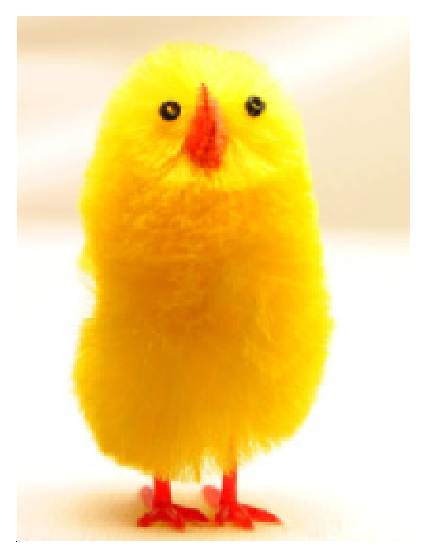
\includegraphics{chick}
\end{center}
\begin{figure}[ht]
  \begin{center}
    \FigureCaptionOpt{My Little Chick!}{My Little Chick}
  \end{center}
\end{figure}

\begin{center}
  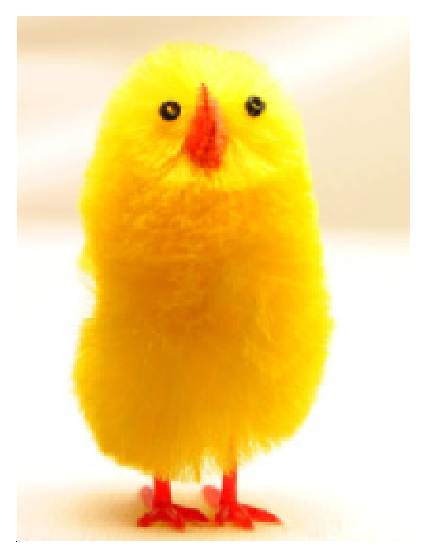
\includegraphics[scale=0.65]{chick}
\end{center}

\begin{figure}[ht]
  \begin{center}
    \FigureCaption{A Resized Figure}
  \end{center}
\end{figure}


\chapter{TESTING FOOTNOTES}
We will now work on testing footnotes.\footnote{This is the first footnote.}
And now let's add some spurious text so that we can have a second\footnote{This
is the second footnote. To test if the footnote is typeset single-spaced, 
we add meaningless text until we can see a second line.} footnote.

\chapter{Generating an Index}
\section{Genereating an Index}
If you want to generate an index, you will need the command \verb=\makeindex[index]= in the 
preamble. Here, index can be any word named by users.\\

The command \verb=\index[index]{entry}= is used to index entry at that point in the document. 
For example, the following code:\\
	\verb=\makeindex[myindex1]= ...\\%
	... Eigenvectors\verb=\index[myindex1]{eigenvector}= ...\\%
will produce output and place the entry `eigenvector' in the myindex1.idx file with the associated page number.\\%

The mcgill etd class redefines the command \verb=\printindex= which should be placed at the point %
in the document where you want your index to appear.And \verb=\printindex= command can be used as following:\\%
  \verb=\printindex[myindex1]{Index - appears in the table of contents}=\\%
  \verb={Index - will be the title of your index.}= \\%
  \verb={Some textual information you want to add the head of your index.}=\\%

Two index formats are defined. One is with leading dots, another is without dots.
If you are also using BIBTEX and index without leading dots, you will need to do:\\
\\
latex filename.tex\\
bibtex filename\\
makeindex -s mcgillpage.ist myindex1 \\
latex filename.tex\\
latex filename.tex\\

\section{Generating a list of abbreviations}
Generating a list of abbreviations is similar to generating an index. Usually, items of an index 
follow by a page number. However, lists of abbreviations do not include page number at all. In this
case, you have to use the following commands to generate a list of abbreviation:\\
	\verb=\makeindex[ListOfAbbr]=\\
	\verb=\index[ListOfAbbr]{WWW@World Wide Web}=\\
	...\\
	\verb=\printindex[ListOfAbbr]{List of Abbreviation}{List of Abbreviation}{}=\\
	
	You need to use makeindex to generate the list as below: \\
	makeindex -s mcgillnopage.ist ListOfAbbr \\
	
	



\chapter{Supporting TexShade}
If you want to use TexShade, you will need to add an option "TexShade" to the 
\verb=\documentclass[optionlist]{mcgilletdclass}=. And it looks like the following: \\
\verb=\documentclass[TexShade, 12pt, letterpaper]{mcgilletdclass}=. Then you should add
the TexShade package into your thesis: \verb=\usepackage{TexShade}=. Here is an example: \\
	\verb=\begin{texshade}{alng.fasta}= \\
	\verb=\noblockskip= \\
	\verb=\hideconsensus= \\
	\verb=\end{texshade}= \\
\\
And you will get the following result:\\%
\begin{texshade}{alng.fasta}
	\noblockskip
	\hideconsensus
\end{texshade}


\SetAppendixName{Appendix}%
\SetAppendixText{Here is the text of an Appendix.  If only one appendix is required, place it here.}%
\ETDAppendix{Appendix A}{Here is the text of an Appendix.}%
\ETDAppendix{Appendix B}{Here is the text of a second, additional Appendix}%
%fjklsdafjklsdafjkldasjfkldjaskl
%\end{\ETDAppendix}%
\bibHeading{References}
\bibliography{mcgilletd}
\bibliographystyle{plain}

\index[abbr]{IEEE@IEEE: Institute of Electrical and Electronics Engineers, Inc.}
\index[abbr]{CDMA@CDMA: code-division multiple access}
\index[abbr]{CTAN@CTAN: comprehensive \protect\TeX{} archive network}


\printindex[keylist]{Index}{Index}{}
\printindex[abbr]{KEY TO ABBREVIATIONS}{KEY TO ABBREVIATIONS}{}

\end{document}


 






